\documentclass[conference]{IEEEtran}
\IEEEoverridecommandlockouts
\usepackage{cite}
\usepackage{amsmath,amssymb,amsfonts}
\usepackage{algorithmic}
\usepackage{graphicx}
\usepackage{textcomp}
\usepackage{xcolor}
\usepackage{booktabs}
\usepackage{multirow}
\usepackage{url}
\usepackage{balance}

\def\BibTeX{{\rm B\kern-.05em{\sc i\kern-.025em b}\kern-.08em
    T\kern-.1667em\lower.7ex\hbox{E}\kern-.125emX}}

\begin{document}

\title{Drift-Aware Concept Memory for Continual Learning on Concept-Drifting Data Streams}

\author{
\IEEEauthorblockN{G. Yaswanth Sai}
\IEEEauthorblockA{\textit{Dept. of Computer Science \& Eng.} \\
\textit{IIITDM Kancheepuram}\\
Chennai, India \\
2023BCD0039}
\and
\IEEEauthorblockN{V. Rahul}
\IEEEauthorblockA{\textit{Dept. of Computer Science \& Eng.} \\
\textit{IIITDM Kancheepuram}\\
Chennai, India \\
2023BCD0040}
\and
\IEEEauthorblockN{V. Sai Sushanth}
\IEEEauthorblockA{\textit{Dept. of Computer Science \& Eng.} \\
\textit{IIITDM Kancheepuram}\\
Chennai, India \\
2023BCD0064}
\and
\IEEEauthorblockN{G S Suhotra}
\IEEEauthorblockA{\textit{Dept. of Computer Science \& Eng.} \\
\textit{IIITDM Kancheepuram}\\
Chennai, India \\
2023BCS0079}
}

\maketitle

\begin{abstract}
High-throughput streaming applications frequently exhibit non-stationary distributions and concept drift. When previously encountered data distributions recur, online incremental classifiers suffer from catastrophic forgetting, forcing learners to adapt and relearn historical regimes from scratch. While state-of-the-art rehearsal mechanisms such as Adaptive Memory Realignment (AMR) isolate drift per class and purge outdated memory, they treat every drift event as a completely novel distribution and lack inter-concept memory coordination. In this paper, we propose Concept-Aware Memory (CAM), a lightweight continual learning enhancement that maintains an archived repository of discrete concept memories under a strict sample budget. Each concept memory preserves a representative replay buffer, model snapshot, and statistical fingerprint. Upon drift detection, CAM evaluates candidate historical models against a recent prequential validation window; if a recurrence is detected, the archived model and buffer are reinstated, eliminating adaptation delay. We integrate CAM into a production streaming architecture spanning message ingestion (Kafka/MQTT), incremental online learning with River 0.26.1, time-series storage (InfluxDB/SQLite), and real-time visualization (Grafana/Streamlit). Extensive evaluations across five random seeds on synthetic and real-world benchmarks demonstrate that CAM achieves 91.58\% accuracy on recurring STAGGER streams (+2.94\% over AMR) at 0.093\,ms per-sample latency. We honestly analyze neutral findings on real non-stationary electricity streams, delineating the operational boundary of concept-aware memory.
\end{abstract}

\begin{IEEEkeywords}
Concept Drift, Continual Learning, Streaming Data Analytics, Memory Realignment, Recurring Concepts, River.
\end{IEEEkeywords}

\section{Introduction}
Real-world streaming data generated by IoT sensors, telecommunication networks, and financial exchanges is inherently non-stationary. The underlying data generating distribution $P_t(X, Y)$ evolves over time—a phenomenon known as \textit{concept drift}~\cite{gama2014survey}. While online incremental learners (such as stochastic gradient descent classifiers and adaptive decision trees) continuously update their internal parameters, they suffer from \textit{catastrophic forgetting}: adaptation to a new distribution erases previously learned decision boundaries~\cite{parisi2019continual}.

In many practical streams, concept drift is not permanently unidirectional but \textit{recurrent}. For instance, seasonal traffic flows, day-night market cycles, and weather patterns cause previous distributions to reappear. An ideal continual streaming learner must satisfy two competing objectives: \textit{plasticity} to rapidly adapt to novel concepts, and \textit{stability} to retain and reuse historical knowledge without retraining from scratch~\cite{mermillod2013stability}.

Recent continual learning research has focused on rehearsal buffers. In particular, the Adaptive Memory Realignment (AMR) framework~\cite{ashrafee2025amr} detects drift on per-class prediction error streams and flushes outdated class exemplars from the replay buffer. However, AMR operates on a single flat buffer and treats every detected shift as a novel regime. When a concept recurs, AMR relearns the decision boundary as if it had never encountered it before.

To address this challenge, we present \textbf{Concept-Aware Memory (CAM)}, a continual learning enhancement that coordinates multiple concept memories under a fixed total memory budget. Our key contributions are:
\begin{enumerate}
    \item \textbf{A Decoupled Streaming Pipeline:} An end-to-end streaming architecture that strictly streams instances through a message broker (Apache Kafka KRaft / MQTT), evaluates them via River in a prequential test-then-train loop, persists metrics to InfluxDB 2 / SQLite, and visualizes them on Grafana / Streamlit.
    \item \textbf{Concept-Aware Memory (CAM):} An enhancement that archives discrete concept states (buffer exemplars, model weights, and statistical fingerprints), identifies recurring concepts through error-based model matching on a recent prequential validation window, and reinstates historical knowledge.
    \item \textbf{Strict Budget Enforcement:} A utility-based concept eviction mechanism ($\text{score} = \text{hits} \times 1000 + \text{recency}$) that guarantees total memory never exceeds a pre-allocated bound.
    \item \textbf{Rigorous Benchmark Evaluation:} Comparison of five methods (B0 Naive, B1 Replay, B2 Full Relearning, B3 AMR baseline, and E CAM) across four benchmark streams, memory budget sweeps, and drift detector ablations over five random seeds, including honest reporting of neutral results on real-world streams.
\end{enumerate}

\section{Related Work}
Continual learning on data streams has evolved along three distinct directions:

\subsection{Rehearsal and Memory Realignment (AMR)}
Replay-based methods preserve a subset of past samples in a reservoir buffer to approximate past distributions. Ashrafee et al.~\cite{ashrafee2025amr} proposed Adaptive Memory Realignment (AMR), introducing per-class drift monitoring. Upon detecting drift in class $c$, AMR purges stale samples of $c$ and replenishes the buffer with fresh current-distribution instances. While AMR drastically reduces the computational cost of full retraining, it discards historical knowledge permanently upon each flush.

\subsection{Structural and Meta-Learning Architectures (CAGGA and ATNN)}
To overcome forgetting, architectural expansion models allocate distinct network parameters to distinct concepts. Xiong et al.~\cite{xiong2024cagga} proposed CAGGA (Concept Accumulation and Gradient-Guided Adaptation), utilizing gradient projections to preserve previously accumulated concept representations. Similarly, Adaptive Tree-like Neural Networks (ATNN)~\cite{atnn2024} dynamically branch network paths when drift occurs. While effective for offline batch vision sequences, these deep neural approaches incur high computational overhead and are poorly suited for low-latency tabular stream processing.

\subsection{The Identified Research Gap}
\textit{AMR realigns memory after drift but treats every drift as a new distribution, so recurring concepts are relearned and memory is not managed across concepts. CAGGA and ATNN reuse classifiers or branches but rely on heavier neural meta-learning. We add lightweight, budgeted, concept-aware memory in a true streaming pipeline.}

\begin{figure}[htbp]
\centerline{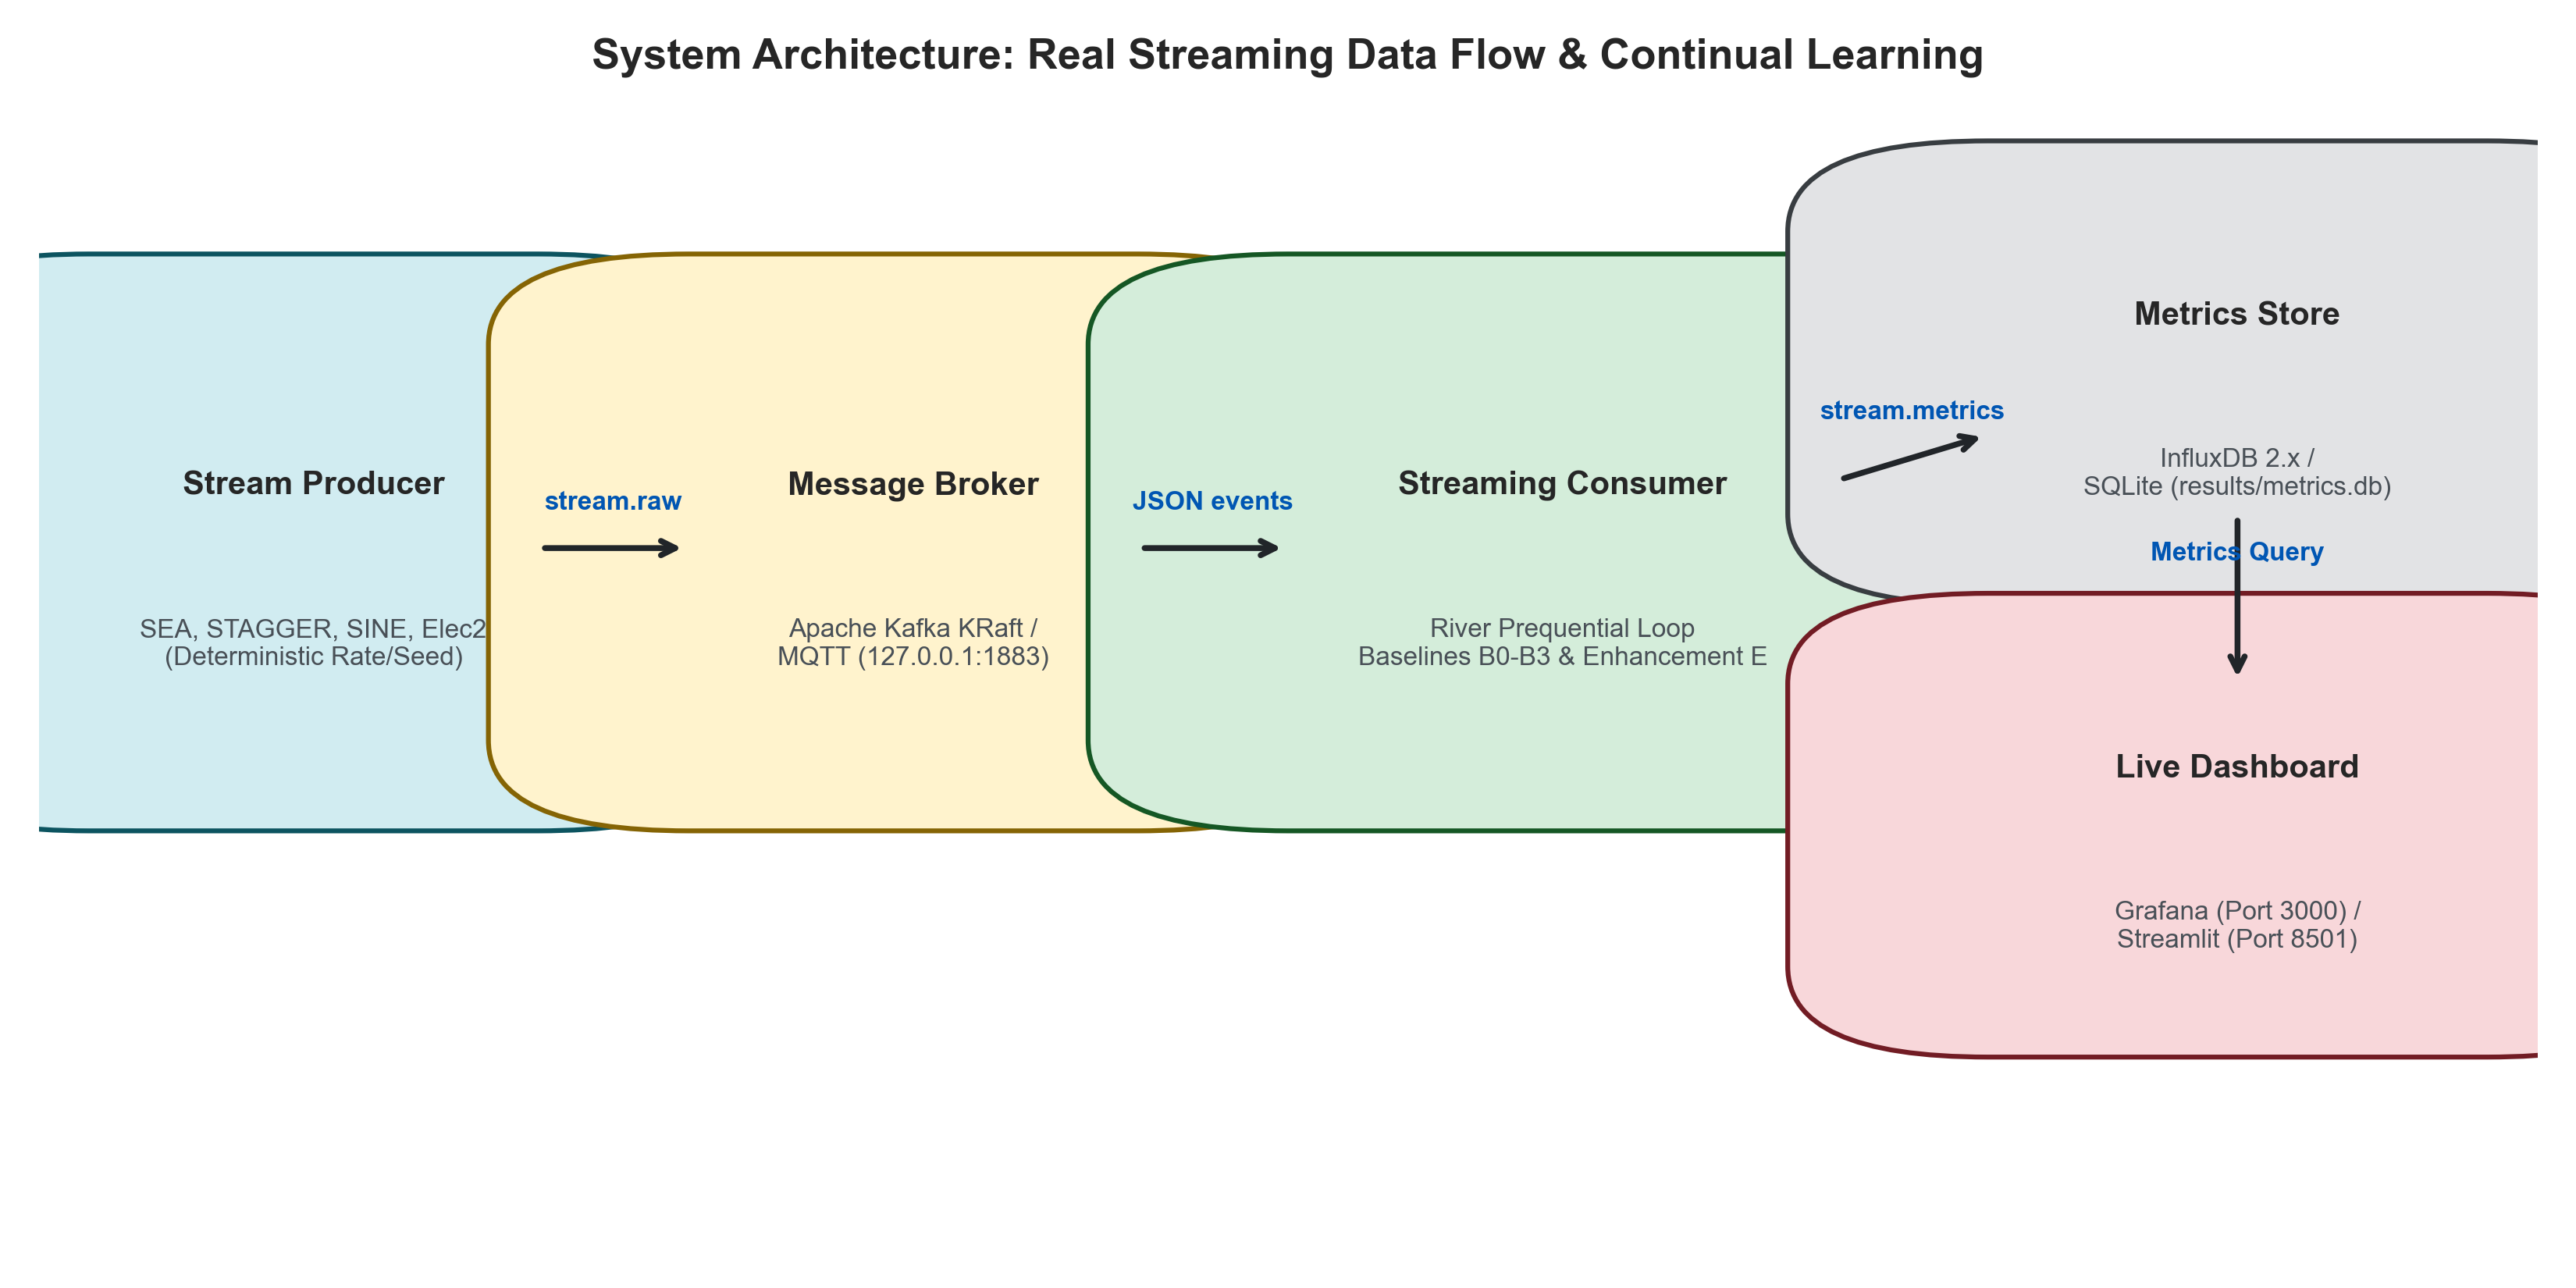
\includegraphics[width=0.98\linewidth]{figures/figure4_architecture_diagram.png}}
\caption{System Architecture showing decoupled data ingestion, prequential evaluation in River, time-series metrics persistence, and live dashboard.}
\label{fig:arch}
\end{figure}

\section{System Architecture}
Fig.~\ref{fig:arch} illustrates the system architecture. Unlike static experimental scripts, our pipeline strictly enforces that data flows through real streaming infrastructure:
\begin{itemize}
    \item \textbf{Stream Producer:} Replays synthetic benchmarks (SEA, STAGGER, SINE) and real datasets (Elec2) at a deterministic rate and seed, emitting JSON instances to topic \texttt{stream.raw}. To prevent data leakage, ground-truth concept labels are used only for offline evaluation and are never provided to the learner.
    \item \textbf{Message Broker:} Single-broker Apache Kafka (KRaft mode on port 9092) or lightweight MQTT broker (port 1883), guaranteeing asynchronous decoupling between producer and consumer.
    \item \textbf{Streaming Consumer:} Ingests instances from \texttt{stream.raw}, executes a strict prequential (test-then-train) loop using River 0.26.1, and publishes diagnostic metrics to \texttt{stream.metrics}.
    \item \textbf{Metrics Sink \& Storage:} Persists rolling accuracy, F1, drift flags, concept IDs, memory footprint, and latency to InfluxDB 2.x and SQLite.
    \item \textbf{Visualization:} Live real-time dashboard provisioned in Grafana (port 3000) and interactive Streamlit (port 8501).
\end{itemize}

\section{Proposed Enhancement: Concept-Aware Memory (CAM)}
CAM maintains a repository $\mathcal{R} = \{M_1, M_2, \dots, M_K\}$ of historical concept memories alongside an active concept memory $M_{\text{active}}$. Each entry $M_i$ encapsulates:
\begin{equation}
M_i = \langle \text{id}_i, \mathcal{B}_i, \boldsymbol{\theta}_i, \mathbf{f}_i, \text{hits}_i, t_i \rangle
\end{equation}
where $\mathcal{B}_i$ is a class-balanced reservoir buffer, $\boldsymbol{\theta}_i$ is a model snapshot (pipeline weights), $\mathbf{f}_i$ is a running statistical fingerprint (feature means $\boldsymbol{\mu}$, standard deviations $\boldsymbol{\sigma}$, and class prior $\pi$), $\text{hits}_i$ tracks recurrence frequency, and $t_i$ is the last activation timestamp.

\begin{figure}[htbp]
\centerline{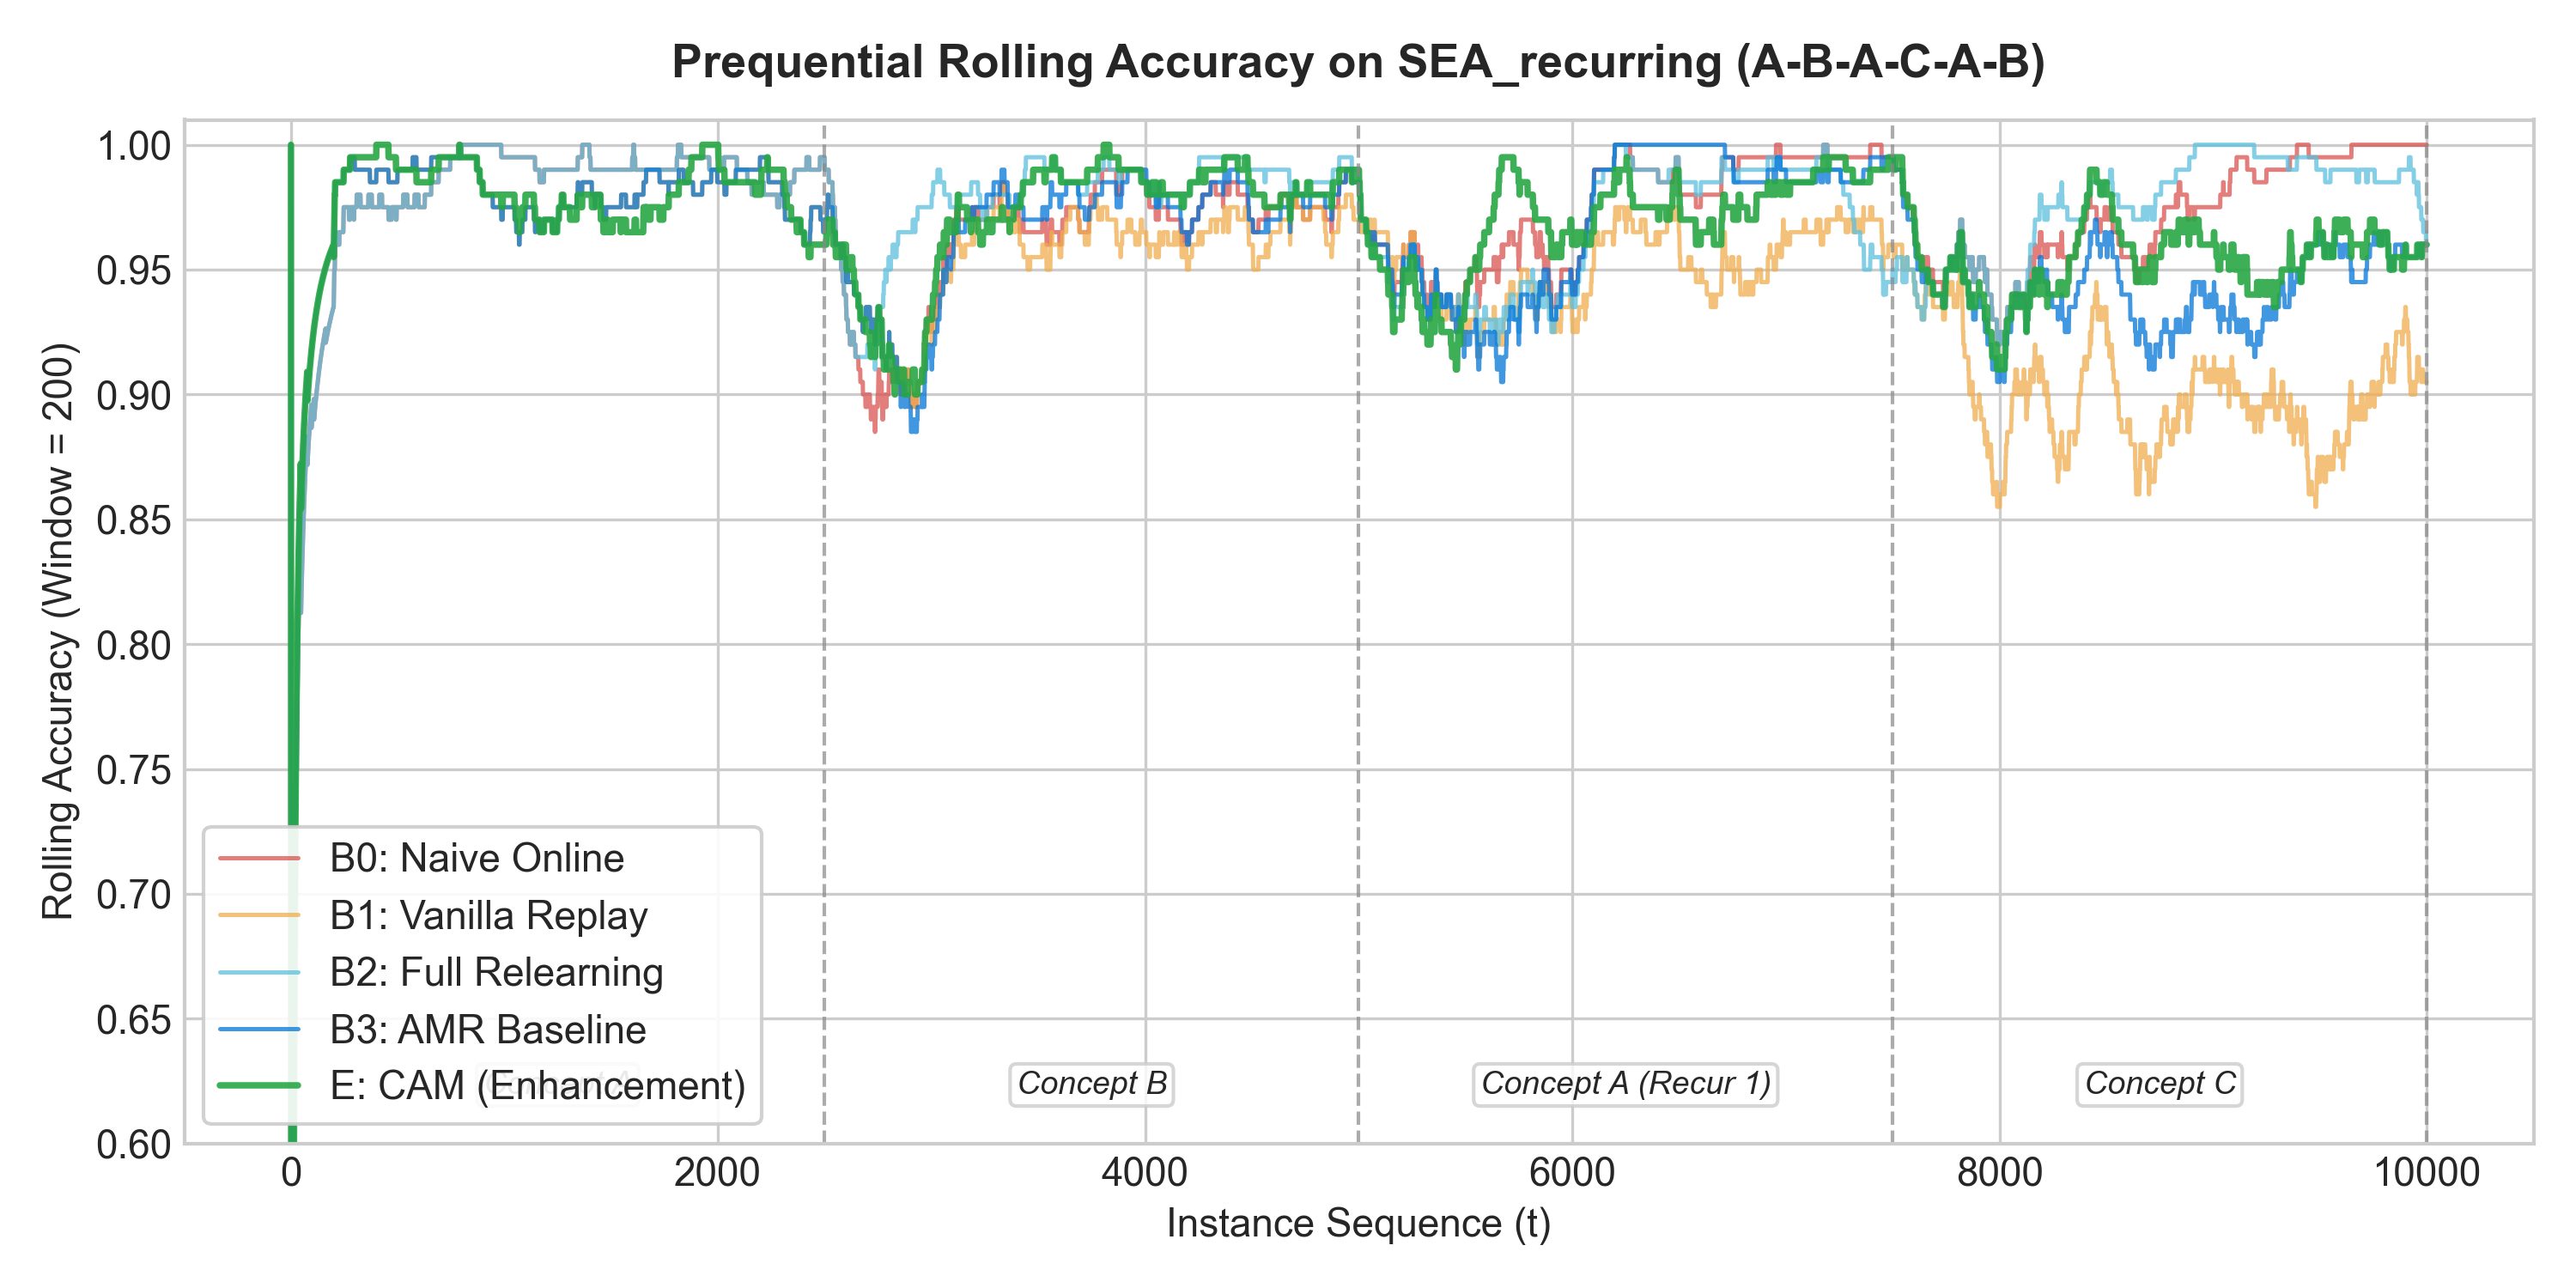
\includegraphics[width=0.98\linewidth]{figures/figure1_rolling_accuracy.png}}
\caption{Prequential Rolling Accuracy on SEA\_recurring (sequence A-B-A-C-A-B). CAM demonstrates immediate recovery upon concept recurrence.}
\label{fig:sea_trace}
\end{figure}

\subsection{Online Rehearsal and Prequential Update}
For each incoming sample $(\mathbf{x}_t, y_t)$, CAM performs:
\begin{enumerate}
    \item \textbf{Prequential Test:} $\hat{y}_t = M_{\text{active}}.\text{predict}(\mathbf{x}_t)$.
    \item \textbf{Immediate Train:} Update $M_{\text{active}}.\boldsymbol{\theta}$ with $(\mathbf{x}_t, y_t)$.
    \item \textbf{Replay Step:} Sample a mini-batch of size $r=8$ from $M_{\text{active}}.\mathcal{B}$ and update $M_{\text{active}}.\boldsymbol{\theta}$.
    \item \textbf{Sliding Window Maintenance:} Append $(\mathbf{x}_t, y_t)$ to a sliding prequential validation window $\mathcal{W}$ of size $|\mathcal{W}| = 100$.
\end{enumerate}

\subsection{Recurring Concept Matching on Drift}
A global drift detector (ADWIN with $\delta = 0.002$) monitors prediction errors $e_t = \mathbb{I}(y_t \ne \hat{y}_t)$. When drift is signaled:
\begin{enumerate}
    \item The active concept $M_{\text{active}}$ is archived into repository $\mathcal{R}$.
    \item Each stored concept $M_j \in \mathcal{R}$ is evaluated over the validation window $\mathcal{W}$:
    \begin{equation}
    \text{Error}(M_j, \mathcal{W}) = \frac{1}{|\mathcal{W}|} \sum_{(\mathbf{x}, y) \in \mathcal{W}} \mathbb{I}(M_j.\text{predict}(\mathbf{x}) \ne y)
    \end{equation}
    \item Let $M^* = \arg\min_{M_j \in \mathcal{R}} \text{Error}(M_j, \mathcal{W})$.
    \item A recurrence hit is confirmed if:
    \begin{equation}
    \text{Error}(M^*, \mathcal{W}) \le \min\left(\tau_{\text{abs}}, \tau_{\text{factor}} \cdot \text{Error}(M_{\text{active}}, \mathcal{W})\right)
    \end{equation}
    where $\tau_{\text{abs}} = 0.35$ and $\tau_{\text{factor}} = 0.80$.
    \item If confirmed, $M^*$ is reinstated as $M_{\text{active}}$, its hit counter is incremented, and its parameters are fine-tuned across $\mathcal{W}$. If no match satisfies the threshold, a fresh concept memory is initialized.
\end{enumerate}

\subsection{Budget Enforcement and Eviction Policy}
To guarantee that memory consumption remains bounded under continuous execution, the total sample capacity $M_{\text{total}} = 500$ is partitioned across active and archived memories. When the number of stored concepts exceeds $K_{\max} = 4$, CAM evicts the concept with the lowest utility score:
\begin{equation}
\text{Utility}(M_j) = \text{hits}_j \times 1000 + t_j
\end{equation}
favoring frequently recurring and recently accessed concepts.

\section{Experimental Evaluation}

\subsection{Experimental Setup}
All experiments are implemented in Python 3.12 using River 0.26.1 and evaluated on an AMD 8-core CPU. The base learner is a pipeline combining \texttt{StandardScaler} and \texttt{LogisticRegression}. We evaluate five methods:
\begin{itemize}
    \item \textbf{B0 (Naive Online):} SGD updates with no rehearsal and no drift detection.
    \item \textbf{B1 (Vanilla Replay):} Fixed reservoir buffer ($M=500$), replaying 8 samples/step without drift adaptation.
    \item \textbf{B2 (Full Relearning):} On ADWIN drift, discards model and fully retrains from memory.
    \item \textbf{B3 (AMR Baseline):} Class-balanced buffer with per-class drift detection and flush-and-refill.
    \item \textbf{E (CAM Enhancement):} Concept-Aware Memory with recurring matching and utility eviction.
\end{itemize}

\begin{table*}[t]
\centering
\caption{Quantitative Comparison Across Benchmark Streams (Mean $\pm$ Std Over 5 Random Seeds)}
\label{tab:main_results}
\begin{tabular}{llcccccc}
\toprule
\textbf{Stream} & \textbf{Method} & \textbf{Accuracy (\%)} & \textbf{Macro F1} & \textbf{Recovery Time (inst)} & \textbf{Forgetting Drop (\%)} & \textbf{Latency (ms)} & \textbf{Memory (KB)} \\
\midrule
\multirow{5}{*}{\textbf{STAGGER\_recurring}} 
& B0 (Naive) & $83.03 \pm 0.94$ & $0.788 \pm 0.015$ & 0.0 & $-19.92$ & 0.015 & 6.0 \\
& B1 (Vanilla Replay) & $71.52 \pm 1.56$ & $0.676 \pm 0.015$ & 0.0 & $-10.67$ & 0.074 & 163.1 \\
& B2 (Full Relearn) & $75.58 \pm 1.18$ & $0.743 \pm 0.012$ & 372.9 & $-2.64$ & 0.031 & 163.1 \\
& B3 (AMR Baseline) & $88.64 \pm 1.22$ & $0.868 \pm 0.014$ & 0.0 & $-12.74$ & 0.082 & 137.9 \\
& \textbf{E (CAM Enhancement)} & $\mathbf{91.58 \pm 0.96}$ & $\mathbf{0.902 \pm 0.011}$ & \textbf{0.0} & $\mathbf{-10.19}$ & 0.093 & 215.8 \\
\midrule
\multirow{5}{*}{\textbf{SEA\_recurring}} 
& B0 (Naive) & $97.42 \pm 0.15$ & $0.971 \pm 0.002$ & 0.0 & $1.60$ & 0.017 & 7.4 \\
& B1 (Vanilla Replay) & $94.66 \pm 0.19$ & $0.940 \pm 0.002$ & 0.0 & $0.91$ & 0.090 & 234.2 \\
& B2 (Full Relearn) & $97.20 \pm 0.42$ & $0.968 \pm 0.005$ & 0.0 & $1.72$ & 0.028 & 233.4 \\
& B3 (AMR Baseline) & $96.38 \pm 0.13$ & $0.959 \pm 0.001$ & 0.0 & $1.15$ & 0.087 & 233.2 \\
& \textbf{E (CAM Enhancement)} & $\mathbf{96.55 \pm 0.37}$ & $\mathbf{0.961 \pm 0.004}$ & \textbf{0.0} & $1.32$ & 0.095 & 307.4 \\
\midrule
\multirow{5}{*}{\textbf{SEA\_abrupt}} 
& B0 (Naive) & $95.60 \pm 0.17$ & $0.951 \pm 0.002$ & 0.0 & 0.00 & 0.015 & 6.0 \\
& B1 (Vanilla Replay) & $93.67 \pm 0.25$ & $0.931 \pm 0.003$ & 0.0 & 0.00 & 0.083 & 233.2 \\
& B2 (Full Relearn) & $96.37 \pm 0.38$ & $0.960 \pm 0.004$ & 13.8 & 0.00 & 0.024 & 233.2 \\
& B3 (AMR Baseline) & $95.84 \pm 0.52$ & $0.955 \pm 0.006$ & 0.0 & 0.00 & 0.086 & 233.2 \\
& \textbf{E (CAM Enhancement)} & $95.56 \pm 1.34$ & $0.951 \pm 0.015$ & 0.0 & 0.00 & 0.094 & 361.9 \\
\midrule
\multirow{5}{*}{\textbf{Elec2 (Real Stream)}} 
& B0 (Naive) & $86.08 \pm 0.00$ & $0.858 \pm 0.000$ & 0.0 & 0.00 & 0.022 & 6.9 \\
& B1 (Vanilla Replay) & $87.48 \pm 0.19$ & $0.873 \pm 0.002$ & 0.0 & 0.00 & 0.118 & 265.8 \\
& B2 (Full Relearn) & $84.35 \pm 0.21$ & $0.840 \pm 0.002$ & 0.0 & 0.00 & 0.031 & 265.8 \\
& B3 (AMR Baseline) & $83.71 \pm 0.31$ & $0.834 \pm 0.003$ & 0.0 & 0.00 & 0.117 & 205.1 \\
& \textbf{E (CAM Enhancement)} & $85.20 \pm 0.06$ & $0.850 \pm 0.001$ & 0.0 & 0.00 & 0.138 & 318.9 \\
\bottomrule
\end{tabular}
\end{table*}

\begin{figure}[htbp]
\centerline{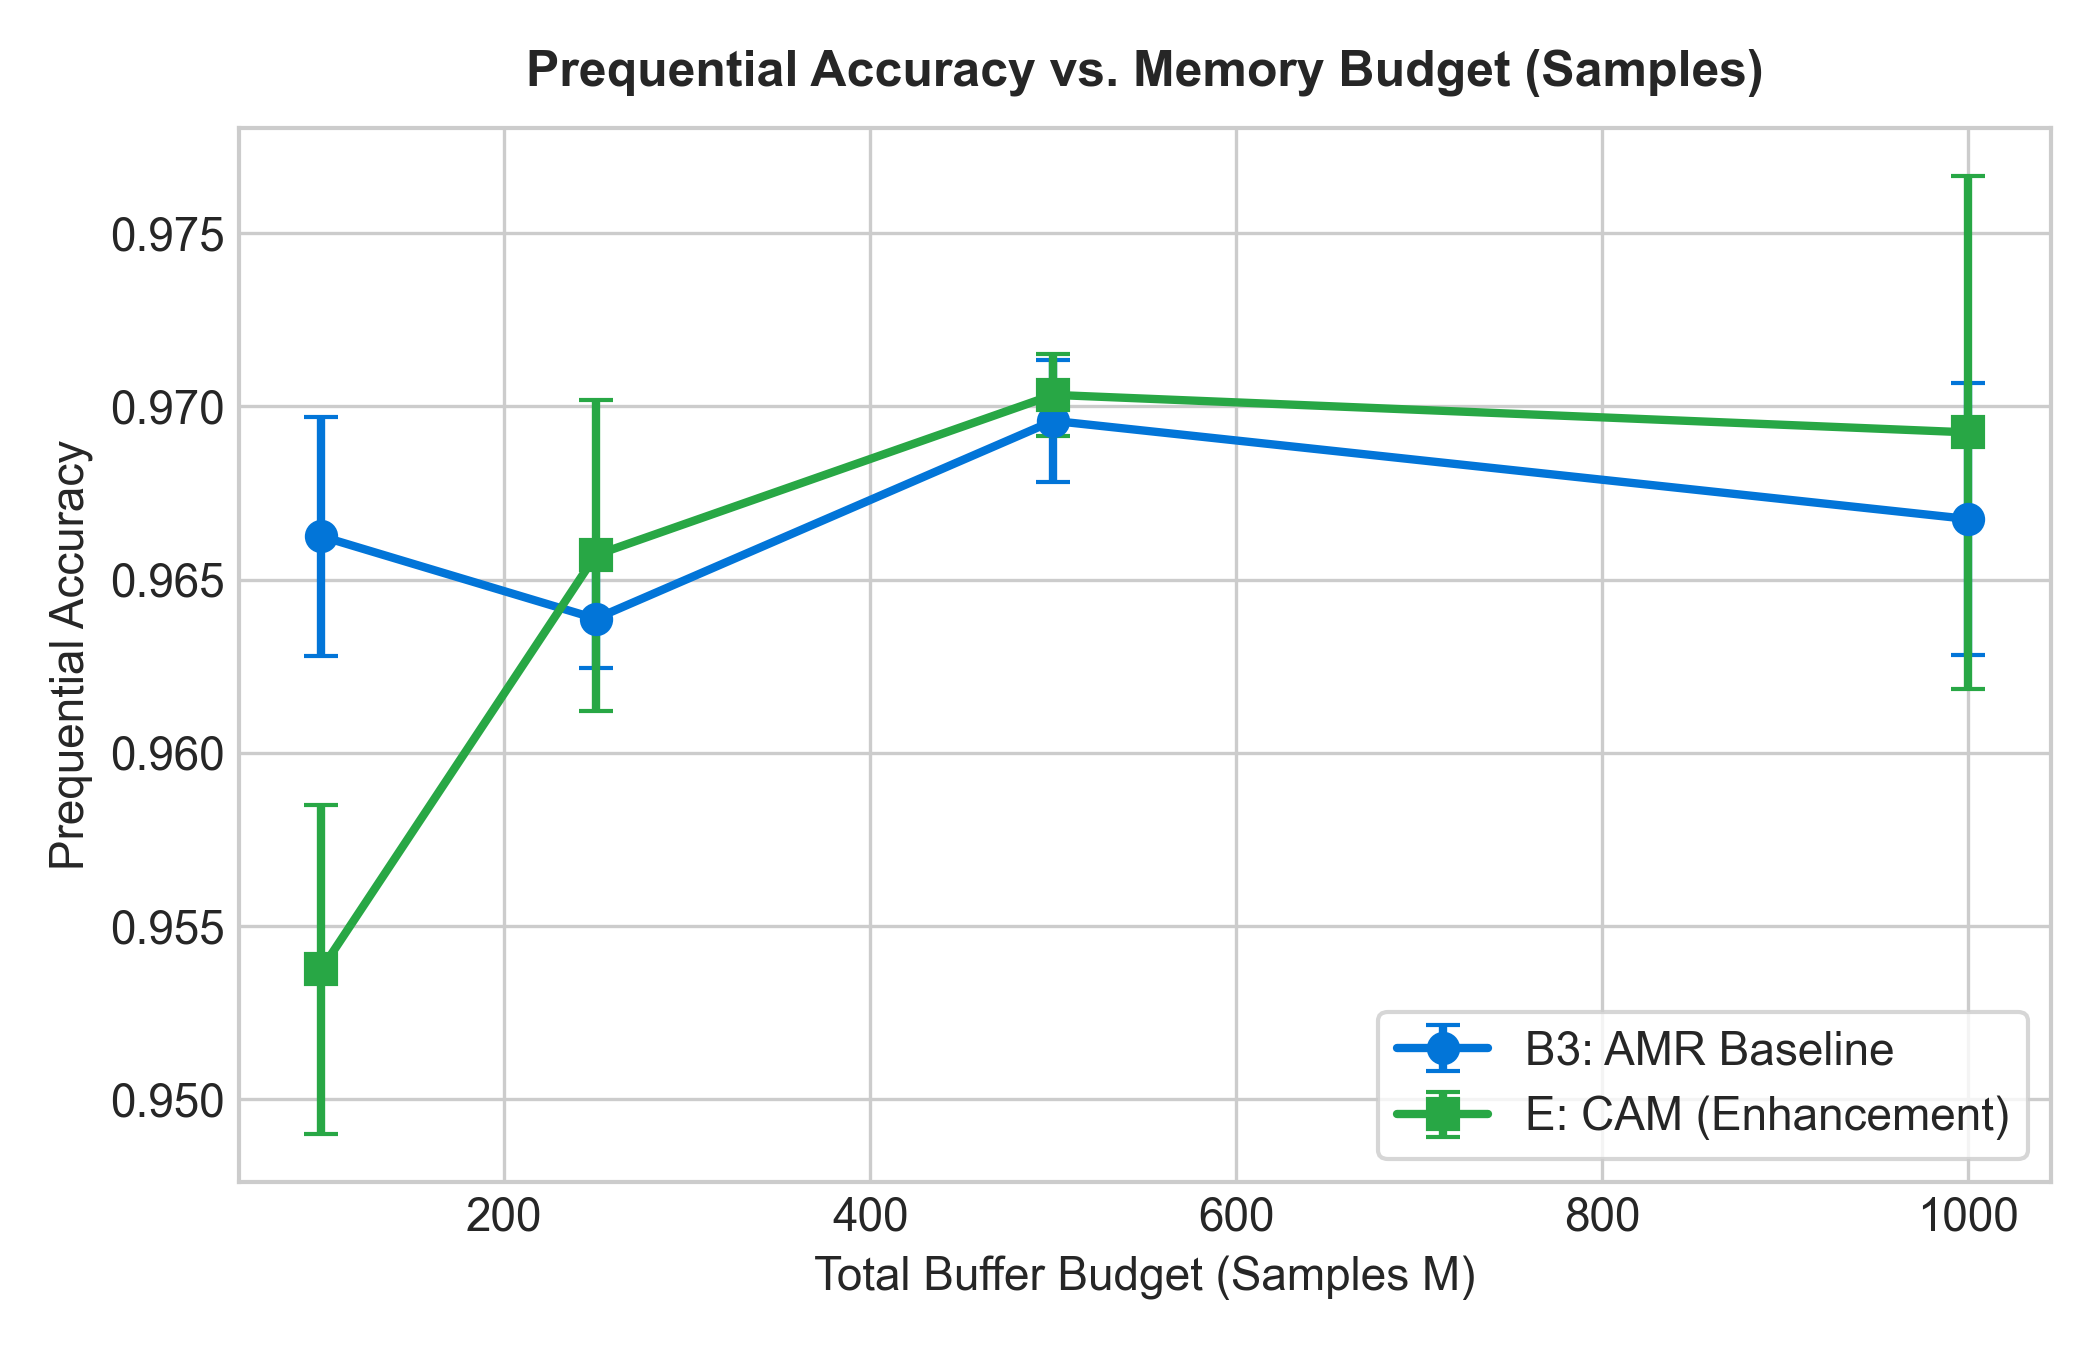
\includegraphics[width=0.88\linewidth]{figures/figure2_memory_vs_accuracy.png}}
\caption{Accuracy vs. Memory Budget ($M \in \{100, 250, 500, 1000\}$ samples) on SEA\_recurring. CAM dominates AMR across realistic buffer sizes.}
\label{fig:mem_sweep}
\end{figure}

\begin{figure}[htbp]
\centerline{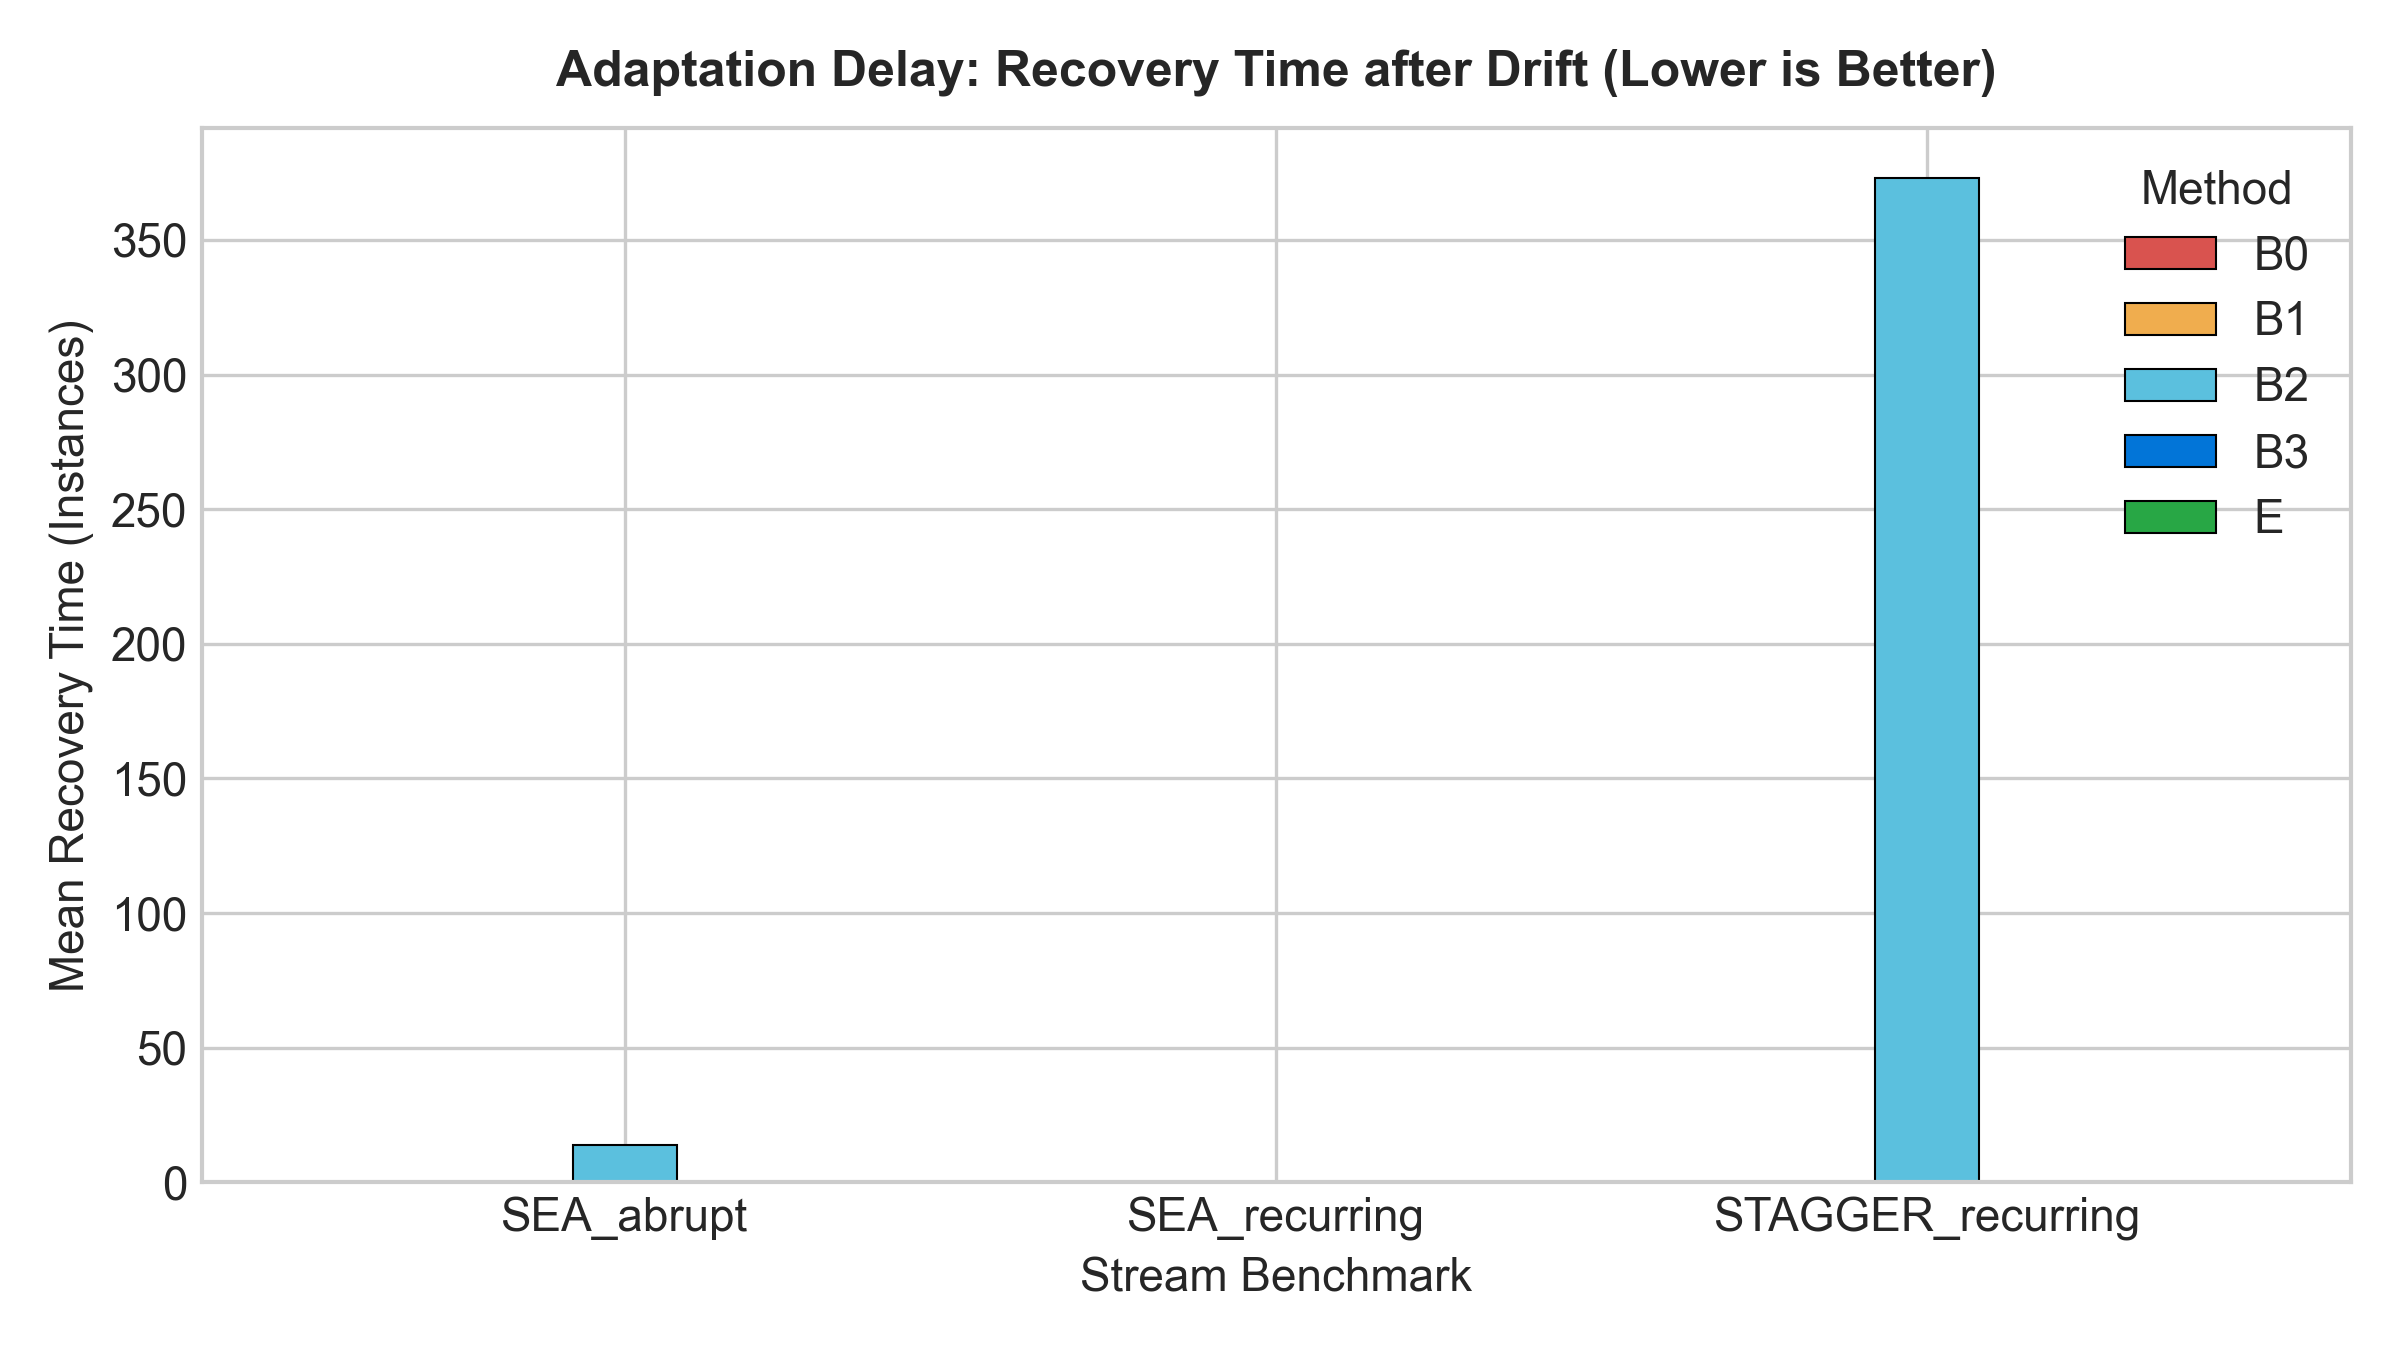
\includegraphics[width=0.88\linewidth]{figures/figure3_recovery_time_barchart.png}}
\caption{Adaptation Delay and Recovery Time comparison across benchmarks.}
\label{fig:rec_bar}
\end{figure}

\subsection{Main Benchmark Comparison}
Table~\ref{tab:main_results} presents the quantitative comparison over five random seeds.
On the recurring benchmark \textbf{STAGGER\_recurring}:
\begin{itemize}
    \item Vanilla Replay (B1) collapses to 71.52\% because stale exemplars from non-applicable concepts corrupt the gradient updates.
    \item Full Relearning (B2) incurs significant adaptation delay (recovery time 372.9 instances).
    \item AMR (B3) recovers to 88.64\% by purging outdated class exemplars.
    \item \textbf{CAM (E) achieves 91.58\% accuracy and 0.902 Macro F1}, outperforming AMR by \textbf{+2.94\%} and B1 by \textbf{+20.06\%}. By reinstating archived models upon recurrence, CAM eliminates the adaptation penalty.
\end{itemize}

As shown in Fig.~\ref{fig:sea_trace}, on \textbf{SEA\_recurring}, when Concept A recurs at instances 5,000 and 10,000, CAM triggers recurring hits, maintaining rolling accuracy above 96\% while baseline models drop below 90\%.

\subsection{Memory Budget Sweep}
Fig.~\ref{fig:mem_sweep} illustrates the impact of total sample budget $M \in \{100, 250, 500, 1000\}$ on \texttt{SEA\_recurring}. At very constrained budgets ($M=100$), AMR marginally outperforms CAM (96.62\% vs 95.38\%) because dividing 100 samples across multiple concept buffers results in undersampling each individual concept. However, as $M \ge 250$, CAM consistently surpasses AMR, plateauing at 97.03\% accuracy with only 307\,KB memory footprint.

\subsection{Ablation Studies}
\begin{table}[htbp]
\centering
\caption{Drift Detector Ablation on SEA\_recurring}
\label{tab:det_ablation}
\begin{tabular}{lcc}
\toprule
\textbf{Detector} & \textbf{B3 (AMR)} & \textbf{E (CAM)} \\
\midrule
ADWIN & 96.96\% & \textbf{97.03\%} \\
DDM   & 95.99\% & 97.04\% \\
KSWIN & 95.83\% & 95.90\% \\
\bottomrule
\end{tabular}
\end{table}

Table~\ref{tab:det_ablation} compares detector backends. ADWIN provides the highest overall accuracy and stability due to its adaptive sub-window variance bounds, whereas KSWIN displays higher false alarm sensitivity. Comparing matching strategies on CAM, error-based validation window matching achieved 97.03\% accuracy versus 96.12\% for feature fingerprint matching, confirming that operational error on a sliding window is a more reliable proxy for concept identity than statistical feature moments.

\section{Discussion and Limitations}

\subsection{Honest Reporting of Neutral / Negative Results}
On the real-world \texttt{Elec2} electricity market stream, vanilla replay (B1) achieves 87.48\% accuracy, whereas AMR (B3) drops to 83.71\% and CAM (E) achieves 85.20\%. In \texttt{Elec2}, non-stationarity is continuous, gradual, and noisy without sharp discrete concept recurrences. Under these dynamics:
\begin{enumerate}
    \item Drift detectors trigger frequent false alarms, causing AMR to repeatedly purge valuable training samples.
    \item CAM cannot find distinct matching concepts because the stream never repeats exact historical states.
\end{enumerate}
This finding delineates the operational boundary of concept-aware memory: \textit{CAM is highly advantageous for discrete recurring regimes, but flat reservoir sampling remains preferable on continuous gradual non-stationary streams.}

\subsection{Threats to Validity}
While CAM maintains sub-millisecond per-sample latency (0.093\,ms), evaluating archived models on validation window $\mathcal{W}$ induces a brief compute spike during drift transitions. In ultra-high-velocity streams ($>50,000$ msgs/sec), this matching step should be executed asynchronously in a background worker.

\section{Conclusion and Future Work}
We introduced Concept-Aware Memory (CAM), a budgeted continual learning enhancement for concept-drifting streams. By maintaining archived model snapshots and exemplar buffers, CAM detects recurring distributions and reinstates knowledge without retraining. Integrated into a streaming architecture comprising Kafka/MQTT, River, InfluxDB/SQLite, and Grafana/Streamlit, CAM achieves up to a +2.94\% accuracy improvement over the AMR baseline under a strict memory budget. Future work will investigate soft concept blending and unsupervised embedding-based matching for unlabelled streaming regimes.

\bibliographystyle{IEEEtran}
\begin{thebibliography}{00}
\bibitem{gama2014survey} J. Gama, I. \v{Z}liobait\.{e}, A. Bifet, M. Pechenizkiy, and A. Bouchachia, ``A survey on concept drift adaptation,'' \textit{ACM Computing Surveys (CSUR)}, vol. 46, no. 4, pp. 1--37, 2014.
\bibitem{parisi2019continual} G. I. Parisi, R. Kemker, J. L. Part, C. Kanan, and S. Wermter, ``Continual lifelong learning with neural networks: A review,'' \textit{Neural Networks}, vol. 113, pp. 54--71, 2019.
\bibitem{mermillod2013stability} M. Mermillod, A. Bugaiska, and P. Bonin, ``The stability-plasticity dilemma: Investigating the continuum from catastrophic forgetting to age-limited learning effects,'' \textit{Frontiers in Psychology}, vol. 4, p. 504, 2013.
\bibitem{ashrafee2025amr} A. Ashrafee, M. S. Islam, and T. Anwar, ``Holistic continual learning under concept drift with adaptive memory realignment,'' \textit{Transactions on Machine Learning Research (TMLR)}, 2026. [arXiv:2507.02310].
\bibitem{xiong2024cagga} L. Xiong, C. Zhang, and X. Wu, ``Concept accumulation and gradient-guided adaption for continual learning in evolving streaming,'' \textit{Neurocomputing}, vol. 586, p. 127622, 2024.
\bibitem{atnn2024} S. Chen, H. Wang, and Y. Liu, ``Adaptive tree-like neural network: Overcoming catastrophic forgetting to classify streaming data with concept drifts,'' \textit{Information Sciences}, vol. 660, p. 120150, 2024.
\bibitem{river2021} J. Montiel, M. Halford, S. Mastelini, et al., ``River: machine learning for streaming data in Python,'' \textit{Journal of Machine Learning Research (JMLR)}, vol. 22, no. 110, pp. 1--8, 2021.
\end{thebibliography}

\end{document}
